\scanpage{47}
% archive sheet number: 46

l) Loi de symétrie autour d'une arête exceptionnelle (comparer au \unsure{ré|n°} fin de e). et structure locale autour d'une composante exceptionnelle de $K$

\figure{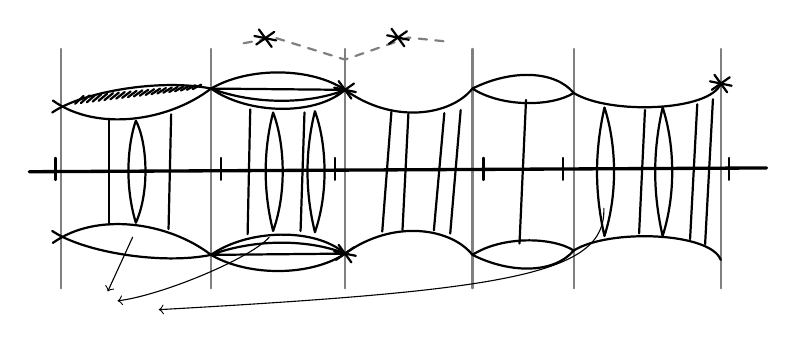
\begin{tikzpicture}[x=.83cm,y=.8cm,line cap=round,line join=round]
\foreach \x in {0,2.3,4.35,6.3,7.85,10.1}{\draw[gray,thick] (\x,-1.85)--(\x,1.95);}
\draw[very thick] (-.48,0)--(10.8,.06);
\foreach \x in {-.08,2.45,4.2,6.47,7.68,10.22}{\draw[thick] (\x,-.13)--(\x,.22);}
\foreach \s in {-1,1}{
\begin{scope}[yscale=\s]
\draw[thick] (-.13,.94) .. controls (.35,1.28) and (1.55,1.48) .. (2.3,1.32) .. controls (2.86,.91) and (3.89,.88) .. (4.35,1.3) .. controls (5.1,.74) and (5.98,.9) .. (6.3,1.32) .. controls (6.75,1.02) and (7.51,1.03) .. (7.85,1.25) .. controls (8.4,.9) and (9.94,.96) .. (10.1,1.4);
\draw[thick] (-.12,1.13) .. controls (.55,.63) and (1.65,.8) .. (2.3,1.32) .. controls (2.88,1.67) and (3.83,1.66) .. (4.35,1.3);
\draw[thick] (2.3,1.32)--(4.35,1.3) (2.3,1.32) .. controls (3,1.05) and (3.83,1.08) .. (4.35,1.3);
\draw[thick] (6.3,1.32) .. controls (6.9,1.63) and (7.56,1.61) .. (7.85,1.25);
\end{scope}}
\foreach \x/\h/\d in {.74/.84/0,1.65/.91/.04,2.86/.99/.04,3.67/.94/.06,4.92/.95/.14,5.23/.92/.09,5.71/.93/.16,5.96/.98/.16,7.02/1.14/.1,8.85/.98/.09,9.63/1.07/.11,9.86/1.15/.12}{\draw[thick] (\x,-\h)--(\x+\d,\h);}
\foreach \x/\h in {1.15/.81,3.25/.94,3.89/.96,8.32/1.02,9.21/1.02}{\draw[thick] (\x,-\h) .. controls (\x-.18,-.2) and (\x-.12,.46) .. (\x,\h) .. controls (\x+.17,.48) and (\x+.22,-.3) .. cycle;}
\foreach \x in {.22,.31,.40,.49,.58,.67,.76,.85,.94,1.03,1.12,1.21,1.30,1.39,1.48,1.57,1.66,1.75,1.84,1.93,2.02}{\draw[thick] (\x,{1.05+.13*\x})--(\x+.13,{1.18+.1*\x});}
\draw[gray,thick,dashed] (2.8,2.04)--(3.27,2.13)--(4.35,1.78)--(5.32,2.13)--(5.97,2.06);
\foreach \x/\y in {3.13/2.12,5.16/2.13,4.35/1.30,4.35/-1.30,10.10/1.40}{\foreach \a in {-55,-12,36}{\draw[thick] (\x,\y)++(\a:.17)--++(\a+180:.34);}}
\draw[thin,->] (1.1,-1.04)--(.72,-1.9);
\draw[thin,->] (3.19,-1.04) .. controls (2.9,-1.38) and (1.55,-1.96) .. (.87,-2.05);
\draw[thin,->] (8.31,-.58) .. controls (8.35,-1.64) and (6.8,-1.88) .. (1.5,-2.19);
\end{tikzpicture}}

figure \unsure{correcte|corrélée|canulée}, \deleted{\unsure{redéjà|il y a}} \unsure{voir|dire} i) j) ---

\margin{\uline{NB} l'indice de chaque arête exceptionnelle stable est \deleted{\unsure{$=$|$\equiv$}} $n-(\nu_{s\unsure{2|1}}-1)-(\nu_{t}-1)$ \deleted{\unsure{$\nu_{s_2}$}} et les instables \deleted{\unsure{$=$|$\equiv$}} $n-v$, où $v$ est la multiplicité du sommet --- où la figure ci-contre est \unsure{concentrée|contractée|constate} ! On voit que l'indice des arêtes exceptionnelles résulte des autres données numériques}

m) Indexation des sections de $L$ sur les faces de $(\mathcal X,K)$ \deleted{à l'aide des} par $\widetilde I$, et passage d'une indexation à l'indexation de la face adjacente

n) Réconstitution de \deleted{$\unsure{\widetilde I|\Sigma}$} $\underline{\Sigma}$ (via $\widetilde I$ \unsure{---|\ldots}) à l'aide de $K$, et des caractères numériques associés à $K$ (indices des \inserted{rd} sommets de $K$, \inserted{$2\nu(s)(-1)^{\unsure{\delta(s)|\varepsilon(s)}}$ où $\nu(s)\in\mathbb N$,} $v(a)$ des arêtes \deleted{ordin\unsure{aires}} de $K$, \deleted{\unsure{et}} (distinguer le cas des arêtes ordinaires et des arêtes exceptionnelles.) Cf aussi

\uline{NB} Il y a aussi sûrement une loi de symétrie autour d'une arête ordinaire, pour ce qui est de la configuration induite par $L$ sur les 2 faces adjacentes, au voisinage de l'arête en question. Peut-être \deleted{un} en tous cas : Considérons la carte $(\mathcal X,K\cup L)$, et ``le voisinage tubulaire stand. et ``\unsure{Thomien|Thurémien|réunion}'' d'arêtes'' de \deleted{$K$ des arêtes} \inserted{son sous-graphe $K$ de} $K\cup L$ dans cette carte. \deleted{considérons} Alors, pour tte $\unsure{a|te}$ arête $a$ de $K$, \unsure{posant|posons}

\figure{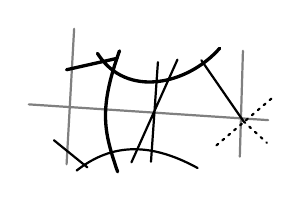
\begin{tikzpicture}[scale=.8,line cap=round]
\draw[gray,thick] (0,-.8)--(.12,1.35) (-.6,.15)--(3.2,-.1) (2.75,-.68)--(2.8,1);
\draw[very thick] (0,.7)--(.8,.88) (.49,.96) .. controls (.95,.23) and (1.93,.47) .. (2.43,1.04);
\draw[very thick] (.84,1) .. controls (.5,.05) and (.6,-.3) .. (.81,-.92);
\draw[thick] (1.45,.82)--(1.34,-.76) (1.76,.86)--(1.03,-.77) (2.14,.85)--(2.81,-.12);
\draw[thick] (-.2,-.42)--(.33,-.85) (.16,-.9) .. controls (.65,-.52) and (1.24,-.4) .. (2.08,-.86);
\draw[dotted,thick] (2.38,-.5)--(3.25,.24) (2.81,-.12)--(3.18,-.46);
\end{tikzpicture}}

$T_a\overset{\mathrm{déf}}{=}(F'\cup F'')\cap T$, où $F',F''$ sont les deux faces de $(\mathcal X,K)$ incidentes à $a$, on a une involution \deleted{\unsure{$\varphi$}} $\sigma_a$ de $a$, ayant en commun un des pts fixes, et respectant la structure cellulaire induite par $(\mathcal X,K\cup L)$. De plus, \deleted{si $a$ et $b$} sont incidentes au m sommet $s$, alors $\sigma_a\mid T_a\cap T_b$ et $\sigma_b\mid T_a\cap T_b$ commutent dans un sens évident
